\chapter{\label{ch:waveletprojection}Wavelet radiosity}
In previous Chapters projection methods and wavelet has been described. Now we describe the use of wavelet basis for projection method and its advantages. 
We first start with the use of wavelet basis for expanding our unknown radiosity function B(x) as linear combination of wavelet basis.\\

$B(x) = b_{\phi_0}\phi_0(x)+\sum_{i,j}^{\inf,\inf}b_{\psi_{i,j}}\psi_{i,j}(x)$\\,
where $b_{\phi_0}$ and $b_{\psi_{i,j}}$ coefficients are inner products\\
$b_{\psi_{i,j}}=<B(x),psi_{i,j}(x)>$
From inner product point of view, we find that the small coefficients occur because wavelet functions have vanishing moments.
\underline{ define vanishing moments}\\

Different wavelet have different vanishing moments. For example Haar wavelet have one vanishing moment. Due to this a function which is nearly constant over the support of wavelet basis function will have coefficient value near 0 corresponding to that wavelet basis function. Similarly linear Legendre multi-wavelets have two vanishing moment, hence function nearly linear will have near 0 coefficient corresponding to that wavelet basis function. This is the advantage of using wavelet basis over box function as basis.\\

Once we project the radiosity function into wavelet basis we need to operate the integral on the projected as discussed in Chapter \ref{ch:projection}.
\begin{figure}[tbh]
\centering{}
\captionsetup{justification=centering}
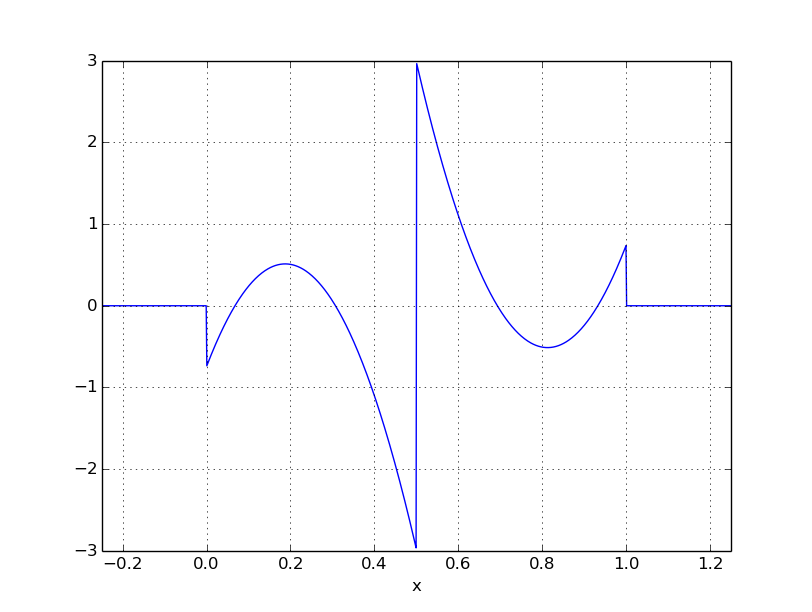
\includegraphics[width=3in]{qlmwpsi2.png}
\caption{\label{fig:f1scene}flatland1 scene: Two parallel segment of length $1$ and $\frac{1}{4}$ apart }
\end{figure}

\begin{figure}[tbh]
\centering{}
\captionsetup{justification=centering}
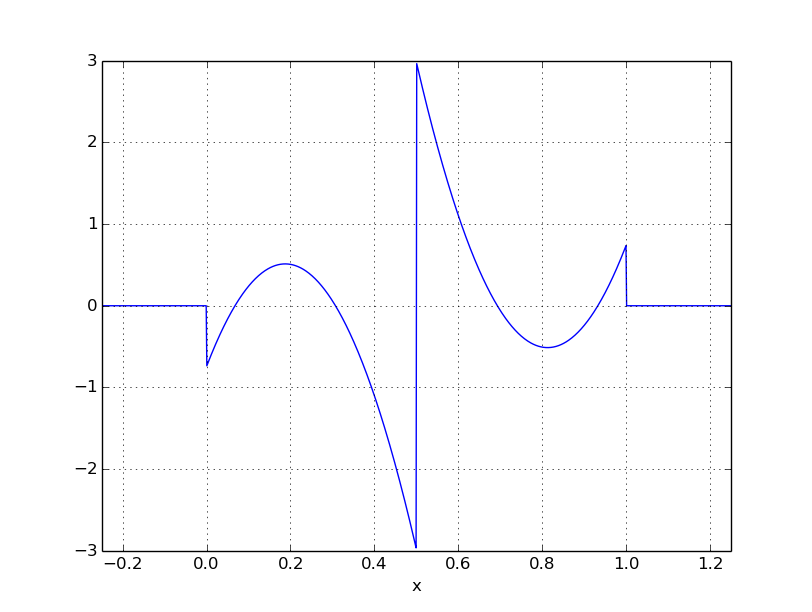
\includegraphics[width=3in]{qlmwpsi2.png}
\caption{\label{fig:f2scene}flatland1 scene: Two parallel segment of length $1$ and $\frac{1}{4}$ apart }
\end{figure}
Consider a 2D scene consisting of the two parallel line segment of length $1$ meter and at distance of $0.25$ meter (see Figure \ref{fig:f1scene}. We divided each segment into 64 equal parts and assume that radiosity function over each part is constant function. Thus we have space of piecewise constant function over the domain of each segment. One of the basis for this space is dilated and translated Haar scaling function (see Chapter \ref{ch:wavelets}). As we have discussed in Chapter \ref{ch:wavelets}, we have alternative basis for the space. This basis is Haar wavelet basis(see Chapter \ref{ch:wavelets}). Figure \ref{fig:haarscalesparsef1} shows the radiosity matrix $K$ with element $K_{i,j}$ obtaned by Equation \ref{eq:kijcalc}, when Haar scaling functions were used for projection. Figure \ref{fig:haarscalesparsef1} shows the radiosity matrix $K$, when Haar wavelet functions were used for projection. Note that each circle represent element. Value of element is proportional to radius of circle corresponding to that element. We can see that just changing the basis of approximation space to wavelet basis, we get very sparse matrix. Some of the elements can be replaced with zero, since many of the elements have value very near to zero. By doing so we will get increased error in projection. But error is very small as compared to sparsity we get after doing so. This sparsity is result of vanishing moments of wavelet. More the vanishing, more will be the sparsity.\\




{\bf explain about the kernel sparsity of wavelet projection }\\
Figure 

\begin{figure}[tbh]
\centering{}
\captionsetup{justification=centering}
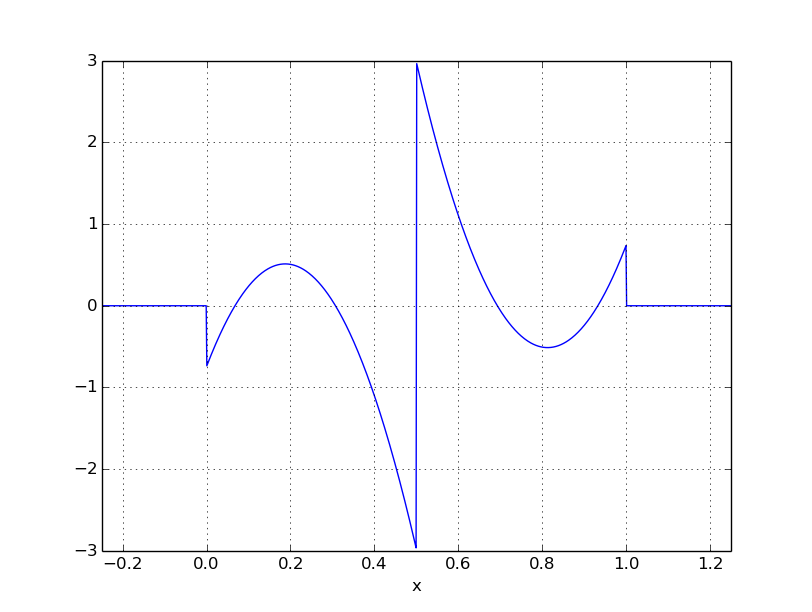
\includegraphics[width=3in]{qlmwpsi2.png}
\caption{\label{fig:haarscalesparsef1}flatland1 with $dist=0.25$ kernel sparsity plot haar scale, radius of circle is proportional to value of element}
\end{figure}
\begin{figure}[tbh]
\centering{}
\captionsetup{justification=centering}
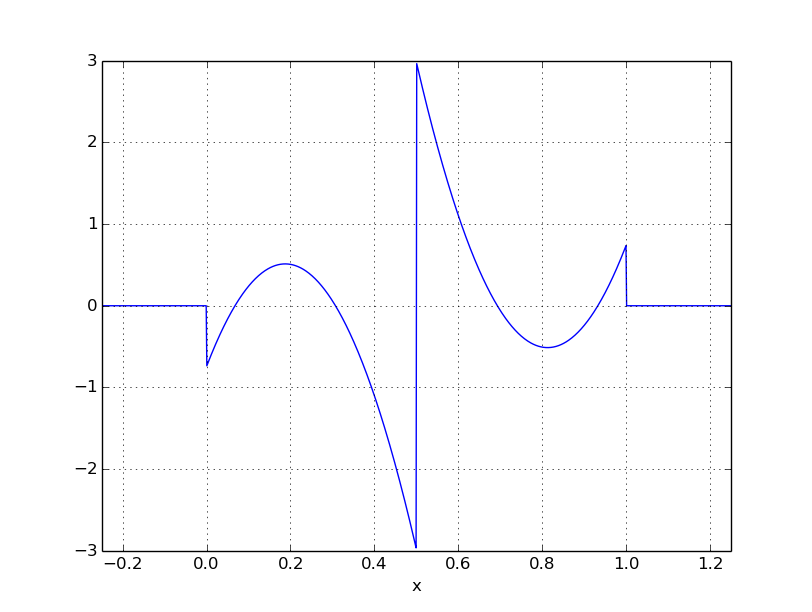
\includegraphics[width=3in]{qlmwpsi2.png}
\caption{\label{fig:haarwaveletsparsef1}flatland1 with $dist=0.25$ kernel sparsity plot haar wavelet}
\end{figure}

Consider another 2D scene consisting of two line segment of length $1$ perpendicular to each other (see Figure \ref{fig:f2scene}. One can see from figure \ref{fig:haarscalesparsef2} and \ref{fig:haarwaveletsparsef2} that similar results are obtained for different 2D scene.

\begin{figure}[tbh]
\centering{}
\captionsetup{justification=centering}
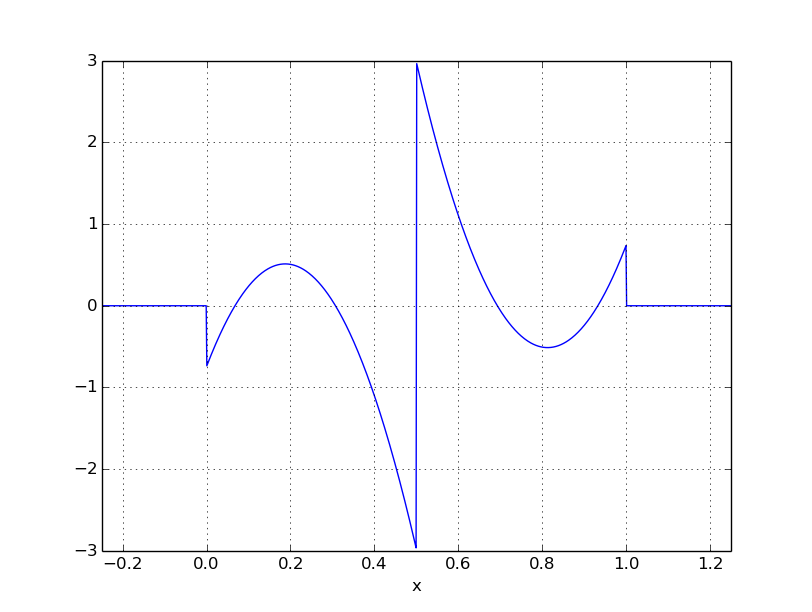
\includegraphics[width=3in]{qlmwpsi2.png}
\caption{\label{fig:haarscalesparsef2}flatland1 with $dist=0.25$ kernel sparsity plot haar scale, radius of circle is proportional to value of element}
\end{figure}
\begin{figure}[tbh]
\centering{}
\captionsetup{justification=centering}
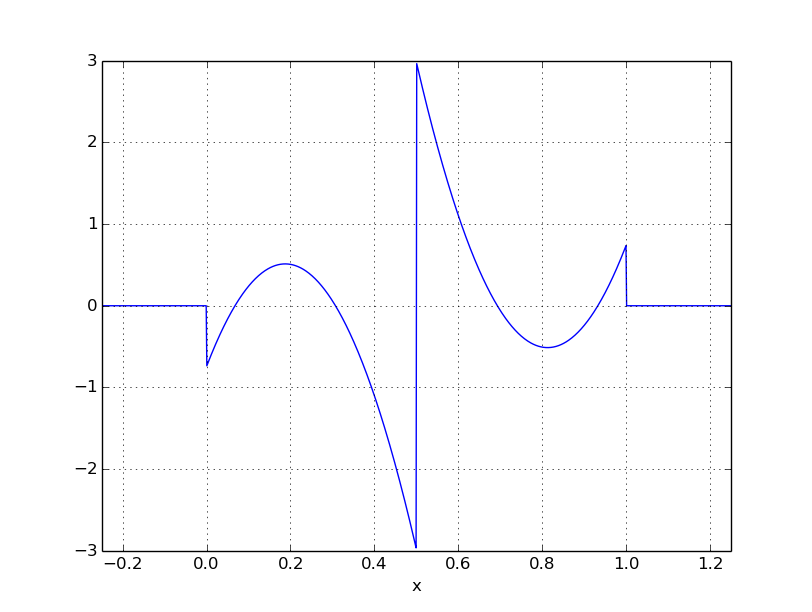
\includegraphics[width=3in]{qlmwpsi2.png}
\caption{\label{fig:haarwaveletsparsef2}flatland1 with $dist=0.25$ kernel sparsity plot haar wavelet}
\end{figure}

\section{Three Dimensional Radiosity and Implementation}
For understanding advantages of wavelet basis we selected 2D scenes. But for 3D scene we need to have 2D basis defined over domain of all 2D surfaces of 3D scene. One simplest way to get 2D wavelet is tensor product of 1D basis. Thus 3D radiosity problem can be solved using projection method with 2D wavelet basis. Coefficients are calculated using Gauss quadrature \cite{stoer}. Thus we need to calculate 4D integral to find coefficient of 4D radiosity matrix $K$. A $p$ point  Gauss-Legendre rule can calculate an accurate integral for polynomials of order up to  $2p-1$.

In next chapter, Chapter \ref{ch:experimentandresult}, we tested wavelet basis with more 2D scenes and also discussed results of 3D radiosity scenes.




\begin{figure}[tbh]
\centering{}
\captionsetup{justification=centering}
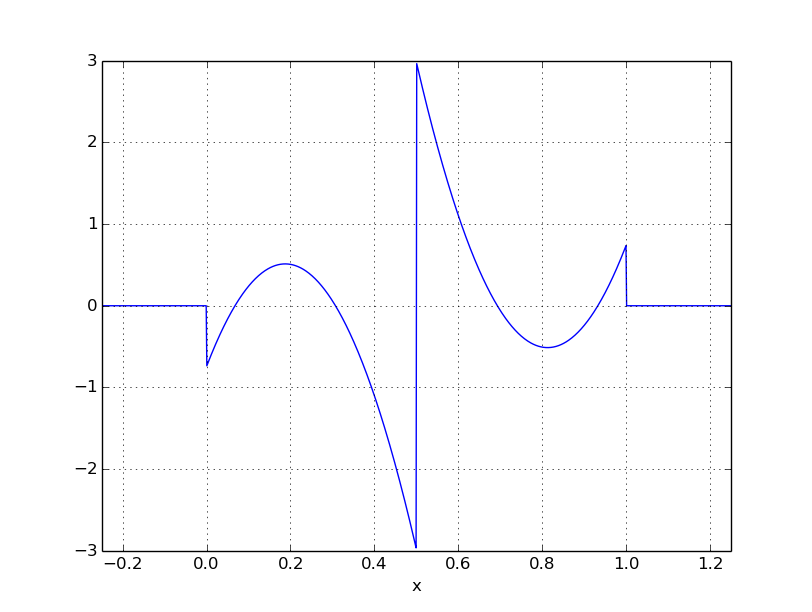
\includegraphics[width=3in]{qlmwpsi2.png}
\caption{\label{fig:replacethis7}flatland1 with $dist=0.25$ kernel sparsity plot llmw wavelet}
\end{figure}

\begin{figure}[tbh]
\centering{}
\captionsetup{justification=centering}
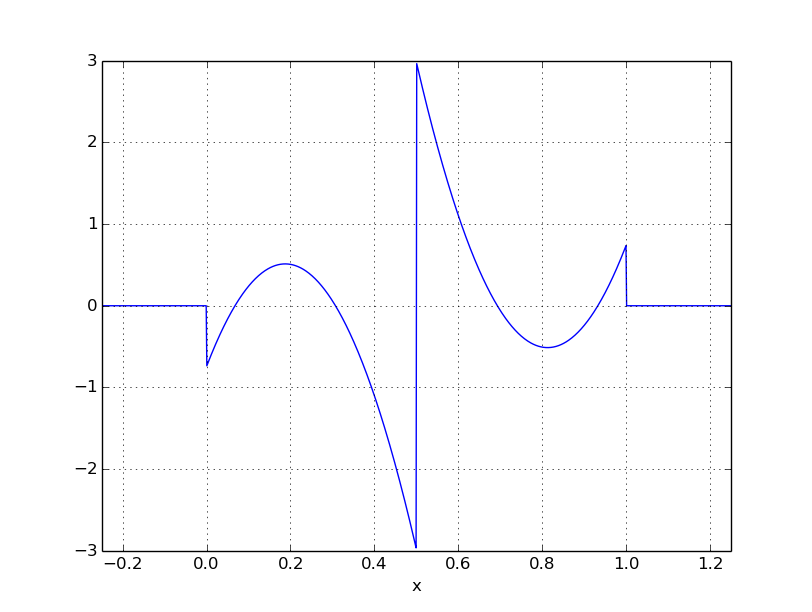
\includegraphics[width=3in]{qlmwpsi2.png}
\caption{\label{fig:replacethis8}flatland1 with $dist=0.25$ kernel sparsity plot qlmw wavelet}
\end{figure}
\underline{discuss about m2 and m3 aswell, also tell about advantage of sparse matrix}

\begin{figure}[tbh]
\centering{}
\captionsetup{justification=centering}
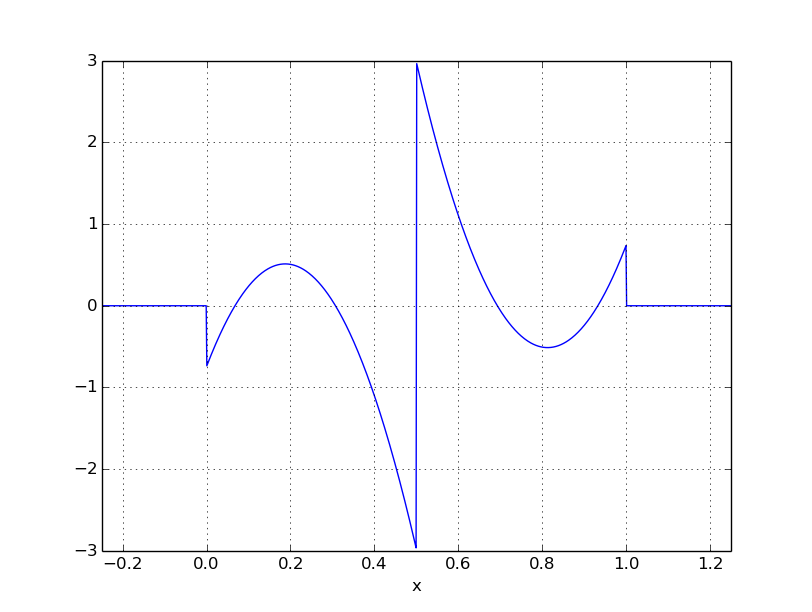
\includegraphics[width=3in]{qlmwpsi2.png}
\caption{\label{fig:replacethis10}flatland2  kernel sparsity plot  llmw wavelet}
\end{figure}

\begin{figure}[tbh]
\centering{}
\captionsetup{justification=centering}
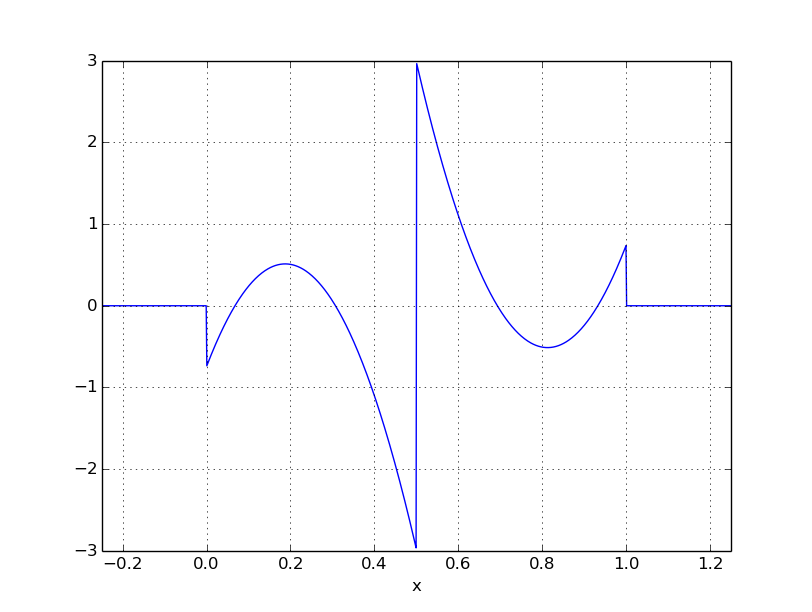
\includegraphics[width=3in]{qlmwpsi2.png}
\caption{\label{fig:replacethis11}flatland2 kernel sparsity plot qlmw wavelet}
\end{figure}

{\bf expalin about 2D and 4d wavelet function (tensor product)}